%Ovo je šablon za generisanje rada za SYMOPIS.

\documentclass[a4paper,serbian]{symopissr}

\usepackage[T1]{fontenc}
\usepackage[utf8]{inputenc}
\usepackage{amsmath,amsthm,amsfonts,amssymb,latexsym}
\usepackage{microtype}%if unwanted, comment out or use option "draft"
\usepackage{pslatex}
\usepackage{units}
\usepackage{listings}
\usepackage[ruled,vlined,croatian,onelanguage]{algorithm2e}
\SetKwInput{KwInput}{Ulaz}                % Set the Input
\SetKwInput{KwOutput}{Izlaz}

\bibliographystyle{apalike}% the recommended bibstyle  

\title{GENERIČKI ALGORITAM KLASTEROVANJA ZASNOVAN NA OPTIMIZACIJI ROJEM ČESTICA\\GENERIC CLUSTER ALGORITHM BASED ON PARTICLE SWARM OPTIMIZATION}
\titlerunning{Primer rada za SYM-OP-IS} %opciono

\author[1]{DENIS ALIČIĆ}
\author[2]{FILIP VIDOJEVIĆ}
\author[3]{DUŠAN DŽAMIĆ}
\author[4]{MIROSLAV MARIĆ}
\affil[1]{Matematički fakultet, 
          Studentski trg 16, Beograd, Srbija,
          denis\char`_alicic@matf.bg.ac.rs}
\affil[2]{Matematički fakultet, 
          Studentski trg 16, Beograd, Srbija,
          filip\char`_vidojevic@matf.bg.ac.rs
}
\affil[3]{Fakultet organizacionih nauka,
		  Jova Ilića 154, Beograd, Srbija,
		  dusan.dzamic@fon.bg.ac.rs}
\affil[4]{Matematički fakultet, 
          Studentski trg 16, Beograd, Srbija,
          maricm@matf.bg.ac.rs}

\keywords{klasterovanje, optimizacija, pso, k-sredina}% obavezno: Molimo Vas navedite 4-5 ključnih reči
\keywordsen{clustering, optimization, pso, k-means}% mandatory: Please provide 4-5 keywords

\begin{document}

\maketitle


\begin{abstract}
U ovom radu je predložen algoritam za rešavanje problema klasterovanja zasnovan na optimaciji rojem čestica \cite{pso}. Osnovna ideja algortima, kao i kod algoritma K sredina, je centroid \cite{kmeans}. Najvažniji parametar algoritma je funkcija kvaliteta klasterovanja koja se optimizuje i time određuje tip klastera. Jedna čestica predstavlja niz centroida dužine k, zadate kao maksimalan broj klastera.
U svakoj iteraciji algoritma se svakoj instanci iz skupa podataka dodeli klaster na osnovu najbližeg centroida. Funkcija udaljenosti se takođe prosleđuje algoritmu i od nje zavisi oblik klastera. Zatim se primenjuje funkcija kvaliteta i na osnovu pozicije najbolje čestice i najbolje pozicije trenutne čestice pomeri centroid svakoj čestici u skladu sa originalnim PSO (eng.~{\em Particle swarm optimization}) algoritmom.\\  
Prikazani su eksperimenti na nekim od najpoznatijih skupova podataka. Predloženi algoritam je nadmašio algoritam K sredina.
\end{abstract}
\bigskip
\begin{abstractEN}
In this paper, an algorithm for solving clustering problems based on particle swarm optimization \cite{pso} is proposed. The basic idea of algorithms, as with the K mean algorithm, is centroid \cite{kmeans}. The most important parameter of the algorithm is the cluster quality function which is optimized and thus determines the type of cluster. One particle represents a series of centroids of length k, given as the maximum number of clusters.
In each iteration of the algorithm, each instance in the data set is assigned a cluster based on the nearest centroid. The distance function is also passed to the algorithm and the shape of the cluster depends on it. Then the quality function is applied and based on the position of the best particle and the best position of the current particle, the centroid moves to each particle in accordance with the original PSO (Particle swarm optimization) algorithm.
Experiments on some of the most well-known data sets are presented. The proposed algorithm surpassed the K mean algorithm.
\end{abstractEN}

\newpage
\section{Uvod}
\label{sec:uvod}
Klasterovanje je jedan od najpopularnijih problema nenadgledanog učenja.
Predstavlja identifikaciju i grupisanje sličnih instanci u datom skupu podataka. Primene ovog metoda su vrlo široke.
Od zamene grupa njihovim predstavnicima zarad smanjenja broja instanci u skupu podataka, do detekcije raznorodnih tkiva na medicinskim snimcima i identifikaciji sličnih grupa korisnika društvenih mreža u svrhu oglašavanja.\\

Obzirom da za mnoge primene nije moguće jednoznačno odrediti šta je dobro klasterovanje, razvijene su različite metode klasterovanja.
Postojeći algoritmi se mogu svrstati u nekoliko kategorija u odnosu na vrstu i broj klastera koji su njihov rezultat.
Nekim metodama se zadaje ciljni broj klastera, dok drugi kao izlaz mogu dati različit broj klastera.
S druge strane, što se tiče vrste klastera koje daju kao izlaz razlikujemo: Globularne, dobro razdvojene, gustinske, hirejarhijske itd.\cite{ml_mladen}\\

Predloženi metod može u zavisnosti od njegovih parametara: funkcije sličnosti i funkcije kvaliteta, koje će biti opisane kasnije, da generiše različite vrste klastera, dok mu se kao poseban parametar zadaje maksimalan broj klastera.
Algoritam je primarno zasnovan na centroidama. Centroid jednoznačno određuje jedan klaster. Pripadnost klasteru jedne instance se određuje na osnovu najbližeg centroida. Centroida ima koliko i klastera.

\section{Klasterovanje kao optimizacioni problem}
\label{sec:klasterovanje}
Kod problema klasifikacije, koji je vid nadgledanog učenja, postoje dobro definisane funkcije koje nam mogu reći kakav je kvalitet dobijenog modela. To su pre svega tačnost i preciznost, mada postoje još neke poput f1 mere i odziva (eng.~{\em recall})  \cite{information}.\\

Klasterovanje je problem nenadgledanog učenja,
 tako da za konkretno grupisanje ne postoje jednoznačne funkcije koje nam sa sigurnošću mogu reći koliko je ono dobro. Ipak, postoje neke funkcije, definisane tokom vremena od raznih istraživača, koje nam mogu dati ocenu kvaliteta klasterovanja \cite{db_index}\cite{ch_score}.

Zanimljivo je primetiti, da iako na prvi pogled ne deluje tako, algoritam K sredina se takođe može posmatrati kao optimizacioni algoritam. Funkcija koju taj algoritam optimizuje je:
%
\begin{equation}
\sum_{i=1}^{k}\sum_{x \in C_i} d(x, c_i)^2,
\end{equation}
%
gde je $d$ rastojanje, najčešće euklidsko, ali može biti i neko drugo, a $c_i$ centroida i-tog klastera. 
\subsection{Funkcije evaluacije}
Slično metrikama koje se koriste za evaluaciju klasifikacionih modela, postoje funkcije koje koriste informaciju o stvarnim klasama da bi ocenile kvalitet klasterovanja. Neke od njih su:
\begin{itemize}
	\item Rand indeks,
	\item Homogenost,
	\item V-mera.
\end{itemize}  

U realnim primenama stvarne klase nisu dostupne, tako da ove funkcije nisu korišćene niti prilikom implementacije algoritma, niti prilikom evaluacije, te ni u radu neće biti dalje razmatrane.\\

Funkcije koje su korišćene prilikom implementacija i eksperimenata su:
\begin{itemize}
	\item Davies-Bouldin indeks \ref{sec:db},
	\item Calinski-Harabasz indeks \ref{sec:ch}.
\end{itemize}

Za izračunavanje ovih funkcija potrebna je informacija o centroidima klastera i dodeli klastera svakoj instanci iz skupa podataka.   

\subsubsection{Davies-Bouldin indeks}
\label{sec:db}
Metrika \cite{db_index} je zadata formulom:
%
\begin{equation}
\frac{1}{c}\sum_{i=1}^{c}\max_{i \neq j} \left( \frac{\sigma_i + \sigma_j}{d(C_i, C_j)} \right),
\end{equation}
%
gde je $c$ broj klastera, $\sigma$ prosečno rastojanje svih instanci unutar jednog klastera od njegovog centroida, $d$ rastojanje, najčešće euklidsko i $C_i$ centroid i-tog klastera.

Minimizacijom ove funkcije po $C_i$ dobijamo grupe koje imaju malo rastojanje unutar istog klastera, a veliko rastojanje između različitih klastera \cite{db_index}.\\ 

Generalno, to je ideja većine ovih funkcija zasnovanih na centroidama, s tim što na različite načine kvantifikuju rastojanja unutar klastera i između različitih klastera. \\

Minimalna vrednost ove funkcije je 0. Treba biti obazriv sa minimizacijom ove funkcije, jer metode sa mogućnošću povećavanja broja klastera, prilikom optimizacije ove mere teže tome da svaka tačka bude pojedinačni klaster.

U situaciji da postoji beskonačno instanci, samim tim i beskonačno klastera jer je svaka instanca poseban klaster, deo funkcije $\frac{1}{c}$ bi težio ka nuli, onda bi i cela funkcija težila minimalnoj vrednosti.

\subsubsection{Calinski-Harabasz indeks}
\label{sec:ch}
Calinski-Harabasz indeks \cite{ch_score} je nešto složeniji za izračunavanje i interpretaciju.\\
Za dati skup podataka $E$, veličine $n_E$, koji se klasteruje u $k$ klastera, vrednost indeksa je definisana formulom:
%
\begin{equation}
s = \frac{tr(B_k)}{tr(W_k)} \times \frac{n_E - k}{k - 1},
\end{equation}
%
gde je $tr(B_k)$ trag matrice disperzije centroida klastera i $tr(W_k)$ trag matrice disperzije unutar pojedinačnog klastera.\\

Matrice se izračunavaju po formulama:
%
\begin{equation}
	B_k = \sum_{q=1}^{k} n_q(c_q - c_E)(c_q - c_E)^T,
\end{equation}
%
\begin{equation} 
	W_k = \sum_{q=1}^{k}\sum_{x \in C_q}(x - c_q)(x - c_q)^T,
\end{equation}
%
gde je $C_q$ skup instanci u klasteru $q$, $c_q$ centroid klastera $q$, $c_E$  centroida celog skupa instanci $E$ i $n_q$ broj instanci u klasteru $q$.\\

Što je ovaj indeks veći, to je klasterovanje bolje, centroidi su udaljeniji, a rastojanja unutar klastera manja.\\
Zbog načina računanja disperzije klastera, koje se računa kao kvadriran zbir udaljenosti instance od centroida, ovaj indeks je generalno veći za konveksne klastere, što je za algoritam koji je predstavljen u ovom radu prednost jer očekivani izlaz algoritma jesu konveksni klasteri.

\subsection{PSO algoritam}
\label{sec:algoritam}
Optimizacioni algoritam je zasnovan na optimizaciji rojem čestica \cite{pso}.
Pseudokod algoritma je prikazan na slici \ref{pseudokod}.
\begin{algorithm}
\SetAlgoLined
\KwResult{Broj klastera $k$, $k$ centroida i dodeljivanje klastera svakoj instanci}
\KwInput{Skup podataka, maksimalan broj klastera $k$, funkcija evaluacije, funkcija udaljenosti}
\KwOutput{Skup podataka sa pripadajucim klasterima, maksimum $k$ centroida}
 inicijalizuj početni roj\;
 odredi najbolju česticu\;
 \While{nije postignut kriterijum zaustavlja}{
  	\ForEach{česticu u roju}{
		Ažuriraj brzinu čestice na osnovu pozicije najbolje čestice i najbolje pozicije trenutne čestice\;
		Promeni poziciju čestice na osnovu izračunate brzine\;
		Na osnovu funkcije udaljenosti odredi pripadnost svakoj instanci skupa odgovarajućem klasteru\;
		Izračunaj funkciju evaluacije na osnovu dodeljenog klasterovanja\;
		\If{nova pozicija bolja od prethodne najbolje pozicije čestice\;}
		{ažuriraj najbolju vrednost trenutne čestice\;}
		\If{nova pozicija bolja od pozicije najbolje čestice\;}
		{ažuriraj poziciju najbolje čestice\;}
	}
 }
 \Return{klasterovanje najbolje čestice, broj klastera i njene centroide}
 
 \caption{PSO algoritam klasterovanja}
 \label{pseudokod}
\end{algorithm}

Osnovnu PSO algoritma čini jedna čestica roja. Čestica predstavlja jedno rešenje optimizacionog problema.
Jednu česticu u algoritmu razvijenom za potrebe ovog rada predstavlja niz centroida klastera.
Centroidi klastera zajedno sa funkcijom blizine predstavljaju jedinstveno određeno rešenje problema klasterovanja. Za svaku instancu skupa nad kojim se vrši klasterovanje se određuje pripadajući klaster kao najbliži centroid koristeći funkciju daljine koja je prosleđena algoritmu kao parametar.
Od prosleđene funkcije daljine (euklidska distanca, kosinusna ili neka druga), zavisi oblik klastera.
Algoritam je generički u smislu izbora funkcije daljine i funkcije evaluacije koja se optimizuje.

Važan deo svakog algoritma optimizacije je njegova sposobnost pretrage širokog prostora rešenja u odnosu na postizanje lokalnog optimuma u nekoj manjoj oblasti. Kod PSO algoritma ovaj problem je rešen korišćenjem dva parametra koji se odnose na kognitivnu i sociološku komponentu.
Kognitivna komponenta čestice daje značajnost njenoj najboljoj poziciji, dok se sociološka komponenta odnosi na najbolju poziciju celog roja.
Menjanjem vrednosti ove dve komponente, koje su realni brojevi, balansira se izmedju nalaženja globalnog i lokalnog optimuma.\\
%\begin{figure}[h!]
	%\begin{center}
	%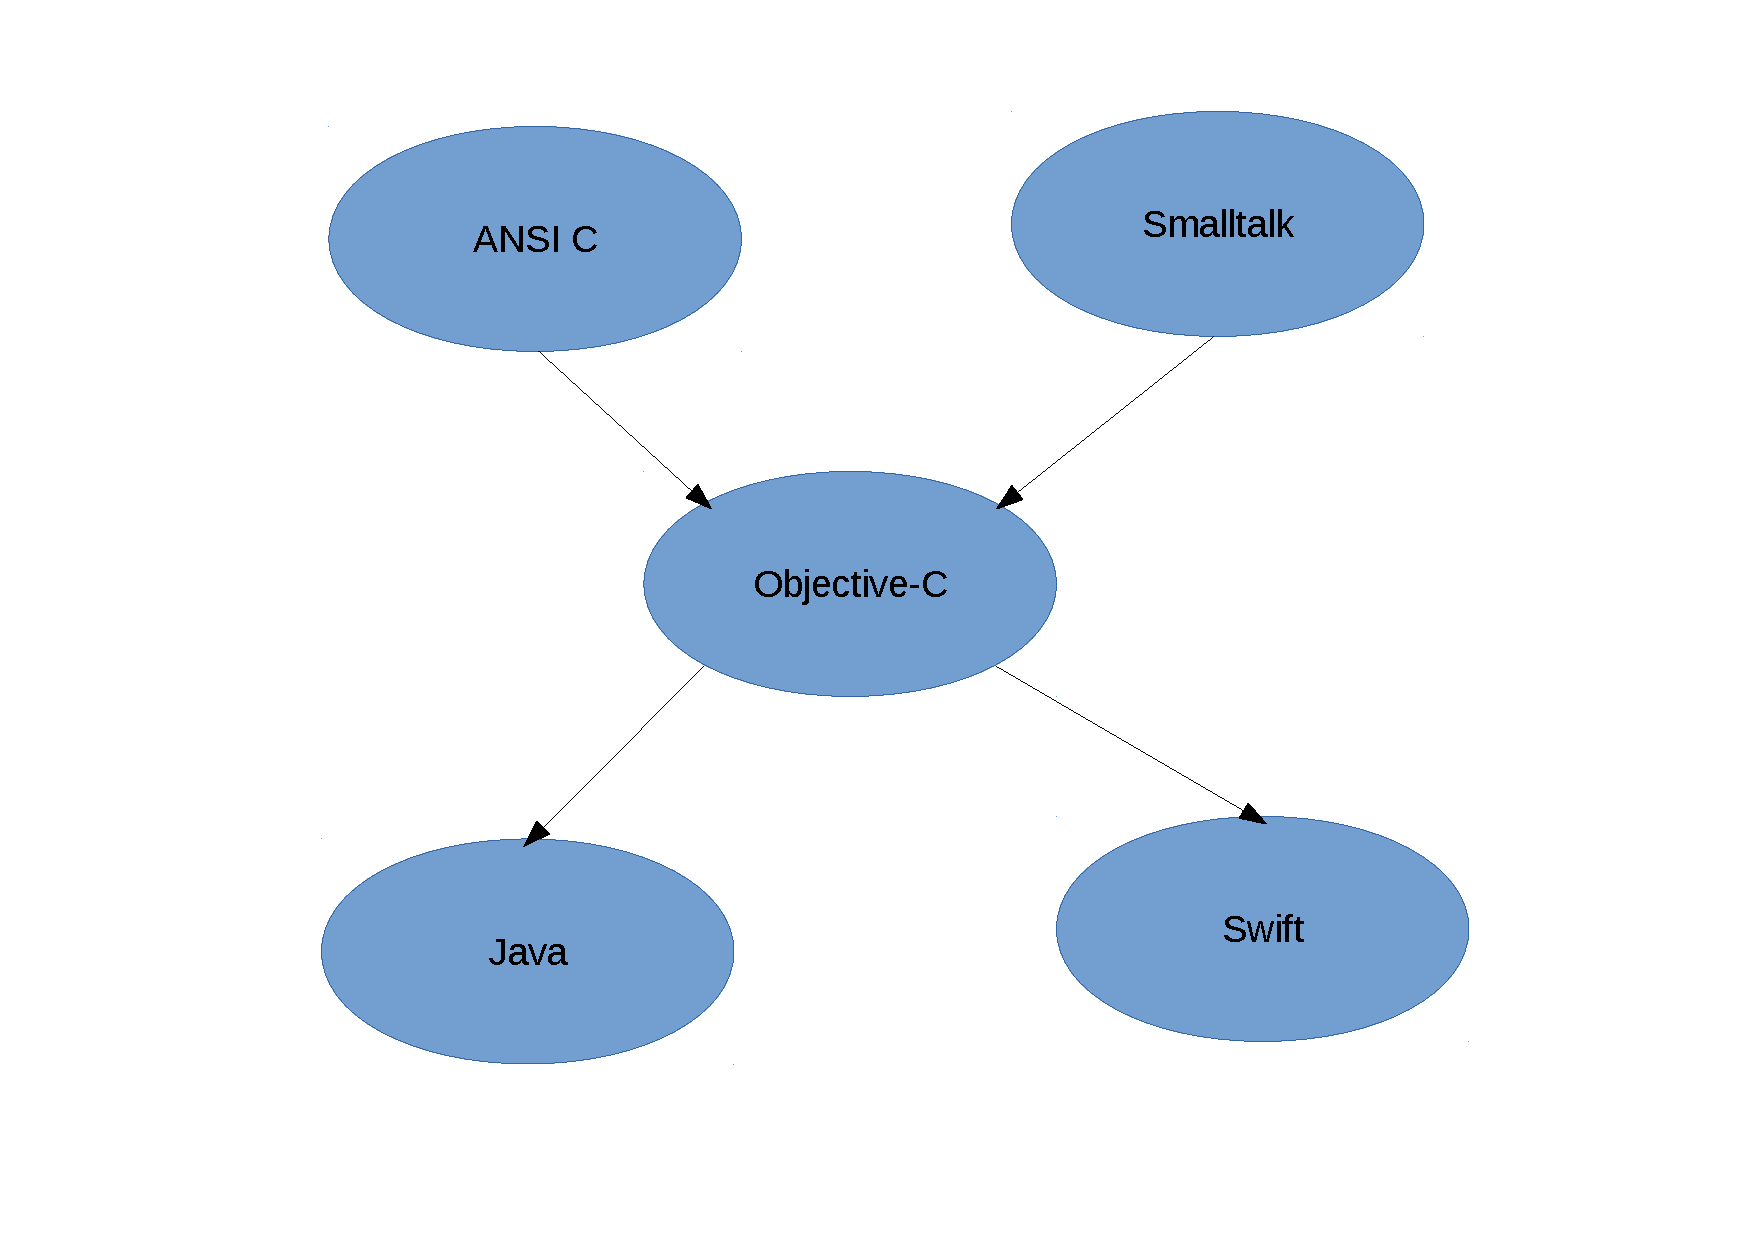
\includegraphics[scale=0.5]{razvojno_stablo}
	%\caption{MVC arhitektura}	
	%\label{fig:MVC}
	%\end{center}
%\end{figure}

\section{Eksperimentalni rezultati}

\label{eksperimenti}
Predloženi algoritam je testiran na poznatim skupovima podataka: IRIS i WINE. U eksperimentima su upoređeni rezultati algoritma K sredina sa PSO algoritmom. Vrednosti prikazane u tabelama \ref{tab:iris} i \ref{tab:wine} predstavljaju vrednosti funkcija evaluacije klasterovanja, koje su detaljno opisane u \ref{sec:db} i \ref{sec:ch}.\\
Za optimizaciju obe funkcije evaluacije korišćenje su vrednosti kognitivne i sociološke komponente, 1 i 2 redom. Taj izbor govori da na jednu česticu više utiče ceo roj, tj. najbolja čestica roja, nego najbolja pozicija trenutne čestice. Veličina roja je 20 čestica i broj iteracija je 500 što je bio i kriterijum zaustavljanja.

\subsection{Iris}
Iris \cite{iris} je jedan od najpoznatijih skupova podataka. Sastoji se od 4 numerička atributa:
\begin{itemize}
	\item dužina krunice,
	\item širina krunice,
	\item dužina čašice,
	\item širina čašice.
\end{itemize} Primarno je namenjen za testiranje algoritama koji rešavaju problem klasifikacije jer sadrži i peti, kategoričli atribut, koji predstavlja vrstu cveta iris. Skup podataka sadrži 3 klase od po 50 instanci. Za potrebe ovog rada iskorišćena su gore navedena četiri atributa bez informacije o pripadajućoj klasi.\\
Zanimljivo je primetiti da je za Davies-Bouldin index \ref{sec:db} broj klastera 2.
U sekciji \ref{sec:algoritam} je naznačeno da se razvijenom algoritmu prosledjuje maksimalan broj klastera i da se taj broj može smanjiti tokom izvršavanja algoritma. Prilikom testiranja algoritma nad ovim skupom podataka za različite parametre kognitivne i sociološke komponente, broja čestica, broja iteracija itd. primećeno je da algoritam kao izlaz da 2 klastera. Analizom skupa podataka je utvrđeno da je jedna klasa linearno razdvojiva od druge dve, što je i navedeno u opisu skupa podataka \cite{uci_iris}.
Tako da se može opravdano pretpostaviti da je ovo jedno od validnih klasterovanja.\\
Očekivano je PSO algoritam nadmašio algoritam K sredina, jer je direktno optimizovao funkcije koje su prikazane u tabeli \ref{tab:iris}.\\

\subsection{Wine}
Skup podataka Wine \cite{uci_wine} je takođe jedan od poznatih skupova. Sastoji se od 13 numeričkih atributa i ciljne klase. Atributi predstavljaju vrednosti različitih hemijskih supstanci do kojih se došlo hemijskom analizom 3 vrste vina koja potiču iz Italije. Skup se sastoji od 178 instanci. Kao i u prethodnom skupu podataka, ni u ovom nije korišćena informacija o klasi.\\
Algoritam je kao parametar prosleđen broj 5 kao maksimalan broj klastera. Prilikom optimizacije obe funkcije, skoro svaki put je algoritam smanjio broj klastera na 3, što itekako ima smisla s obzirom da u skupu podataka zaista postoje 3 klase i za taj broj klastera su funkcije bila minimalne. To takođe znači da su izabrane funkcije pogodne za rešavanje problema klasterovanja nad ovim skupom.\\
Skup podataka Wine se smatra za jedan od lakših primera problema klasifikacije, ali treba imati u vidu da je ovde reč o klasterovanju i da algoritam prilikom izvršavanju ni na koji način nije imao informaciju od broju klasa.\\
U tabeli \ref{tab:wine} su prikazani rezultati izvršavanja PSO algoritma i algoritma K sredina. Očekivano, PSO je i u ovom slučaju nadmašio K sredina.

% Please add the following required packages to your document preamble:
% \usepackage{multirow}
\begin{table}[]
\begin{tabular}{|l|c|c|c|c|}
\hline
\multirow{3}{*}{\textbf{Algoritam}}      & \multicolumn{4}{c|}{\textbf{IRIS}}                                        \\ \cline{2-5} 
                                         & \multicolumn{2}{c|}{\textbf{DB}} & \multicolumn{2}{c|}{\textbf{CZ}} \\ \cline{2-5} 
                                  
     & c         & index                & c & index                                \\ \hline
\multicolumn{1}{|c|}{\textbf{K Sredina}} & 2         & 0.40                & 3 & 561.62                               \\ \hline
\multicolumn{1}{|c|}{\textbf{PSO}}       & 2         & \textbf{0.28}        & 3 & \multicolumn{1}{l|}{\textbf{601.05}} \\ \hline
\end{tabular}
\caption{\label{tab:iris}Vrednosti funkcija evaluacije nad skupom podataka IRIS.}
\end{table}

\begin{table}[]
\begin{tabular}{|l|c|c|c|c|}
\hline
\multirow{3}{*}{\textbf{Algoritam}}      & \multicolumn{4}{c|}{\textbf{WINE}}                                        \\ \cline{2-5} 
                                         & \multicolumn{2}{c|}{\textbf{DB}} & \multicolumn{2}{c|}{\textbf{CZ}} \\ \cline{2-5} 
                                         & c         & index                & c & index                                \\ \hline
\multicolumn{1}{|c|}{\textbf{K Sredina}} & 3         & 0.53                & 3 & 561.81                               \\ \hline
\multicolumn{1}{|c|}{\textbf{PSO}}       & 3         & \textbf{0.43}        & 3 & \multicolumn{1}{l|}{\textbf{585.38}} \\ \hline
\end{tabular}
\caption{\label{tab:wine}Vrednosti funkcija evaluacije nad skupom podataka WINE.}
\end{table}

\section{Zaključak}
\label{sec:zakljucak}
U ovom radu predložen je PSO algoritam za rešavanje problema klasterovanja i predstavljeni su rezulati nad skupovima podataka Iris \cite{iris} i Wine \cite{uci_wine}. Predloženi su parametri razvijenog algoritma zasnovanog na optimizaciji rojem čestica za koje su dobijeni najbolji rezultati nad oba skupa podataka. Razvijeni algoritam je generički u smislu izbora funkcije koja je optimizuje i funkcije blizine dve instance, što omogućava da algoritam kao izlaz ima različite oblike i vrste klastera. Takođe, algoritam se može koristiti za određivanje broja klastera.\\
Buduća istraživanja bi bila usmerena ka hibridizaciji algoritma sa drugim poznatim heurističkim algoritmima globalne optimizacije.

%%
%% Bibliografija
%%

\begin{thebibliography}{99}

\bibitem{kmeans} Stuart P. Lloyd (1982). Least squares quantization in pcm.
    IEEE Transactions on Information Theory, 129-137 vol 28.
\bibitem{pso} Kennedy, J. and Eberhart, R. (1995). Particle swarm optimization. Proceedings of ICNN'95 - International Conference on Neural Networks, 1942-1948 vol.4.
\bibitem{ch_score} Harabasz, Calinski T and Karo{\'n}ski, M. (1974). Communications in Statistics - A dendrite method for cluster analysis, 1-27 vol. 3.  
\bibitem{db_index} David L. Davies and D. Bouldin (1979). A Cluster Separation Measure. IEEE Transactions on Pattern Analysis and Machine Intelligence, 224-227 vol. PAMI-1.
\bibitem{iris} Edgar Anderson (1936). The Species Problem in Iris. Annals of the Missouri Botanical Garden, 457-509, vol. 23.
\bibitem{ml_mladen} Nikolić M. (2019). Mašinsko učenje.  
	http://ml.matf.bg.ac.rs/readings/ml.pdf.
\bibitem{uci_iris} UCI Machine Learning repository: Iris data. https://archive.ics.uci.edu/ml/datasets/iris, accessed: 2021-06-14.
\bibitem{uci_wine} UCI Machine Learning repository: Wine data. https://archive.ics.uci.edu/ml/datasets/wine, accessed: 2021-06-14.
\bibitem{information} Jones, K Sparck and Van Rijsbergen, Cornelis Joost (1976). Information retrieval test collections. Journal of documentation, MCB UP Ltd.
\end{thebibliography}


\end{document}
